% Generated by analysis/judge_figures.py - do not edit by hand.
\definecolor{cert}{HTML}{2A78D6}\definecolor{ink2}{HTML}{52514E}
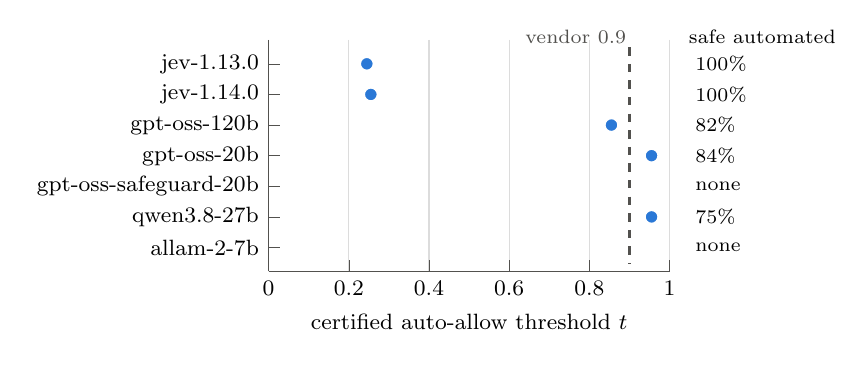
\begin{tikzpicture}
\begin{axis}[scale only axis, width=0.42\columnwidth, height=2.94cm,
  xmin=0, xmax=1, xtick={0,0.2,0.4,0.6,0.8,1}, xlabel={certified auto-allow threshold $t$},
  xlabel style={font=\footnotesize},
  symbolic y coords={jev-1.13.0,jev-1.14.0,gpt-oss-120b,gpt-oss-20b,gpt-oss-safeguard-20b,qwen3.8-27b,allam-2-7b}, ytick={jev-1.13.0,jev-1.14.0,gpt-oss-120b,gpt-oss-20b,gpt-oss-safeguard-20b,qwen3.8-27b,allam-2-7b}, y dir=reverse, enlarge y limits=0.13,
  ymin=jev-1.13.0, ymax=allam-2-7b,
  clip=false, axis line style={ink2}, tick style={ink2}, ticklabel style={font=\footnotesize},
  xmajorgrids, grid style={ink2!20}, axis x line*=bottom, axis y line*=left]
\draw[ink2, dashed, thick] (axis cs:0.9,jev-1.13.0) ++(0pt,6pt) coordinate (top)
  (axis cs:0.9,allam-2-7b) ++(0pt,-6pt) coordinate (bot) (top) -- (bot);
\node[anchor=south east,font=\scriptsize,text=ink2,inner sep=1pt] at (top) {vendor 0.9};
\node[above,font=\scriptsize,anchor=south west,inner sep=1pt] at (axis cs:1.04,jev-1.13.0) [yshift=6pt] {safe automated};
\addplot[only marks, mark=*, mark size=2.4pt, color=cert, mark options={draw=white, line width=0.6pt}]
  coordinates {(0.245,jev-1.13.0) (0.255,jev-1.14.0) (0.855,gpt-oss-120b) (0.955,gpt-oss-20b) (0.955,qwen3.8-27b)};
\node[anchor=west,font=\scriptsize] at (axis cs:1.04,jev-1.13.0) {100\%};
\node[anchor=west,font=\scriptsize] at (axis cs:1.04,jev-1.14.0) {100\%};
\node[anchor=west,font=\scriptsize] at (axis cs:1.04,gpt-oss-120b) {82\%};
\node[anchor=west,font=\scriptsize] at (axis cs:1.04,gpt-oss-20b) {84\%};
\node[anchor=west,font=\scriptsize] at (axis cs:1.04,gpt-oss-safeguard-20b) {none};
\node[anchor=west,font=\scriptsize] at (axis cs:1.04,qwen3.8-27b) {75\%};
\node[anchor=west,font=\scriptsize] at (axis cs:1.04,allam-2-7b) {none};
\end{axis}
\end{tikzpicture}
